\section{CTimer\-Event::CTimer\-Generic\-Reactor  Class Reference}
\label{classCTimerEvent_1_1CTimerGenericReactor}\index{CTimerEvent::CTimerGenericReactor@{CTimer\-Event::CTimer\-Generic\-Reactor}}
Inheritance diagram for CTimer\-Event::CTimer\-Generic\-Reactor::\begin{figure}[H]
\begin{center}
\leavevmode
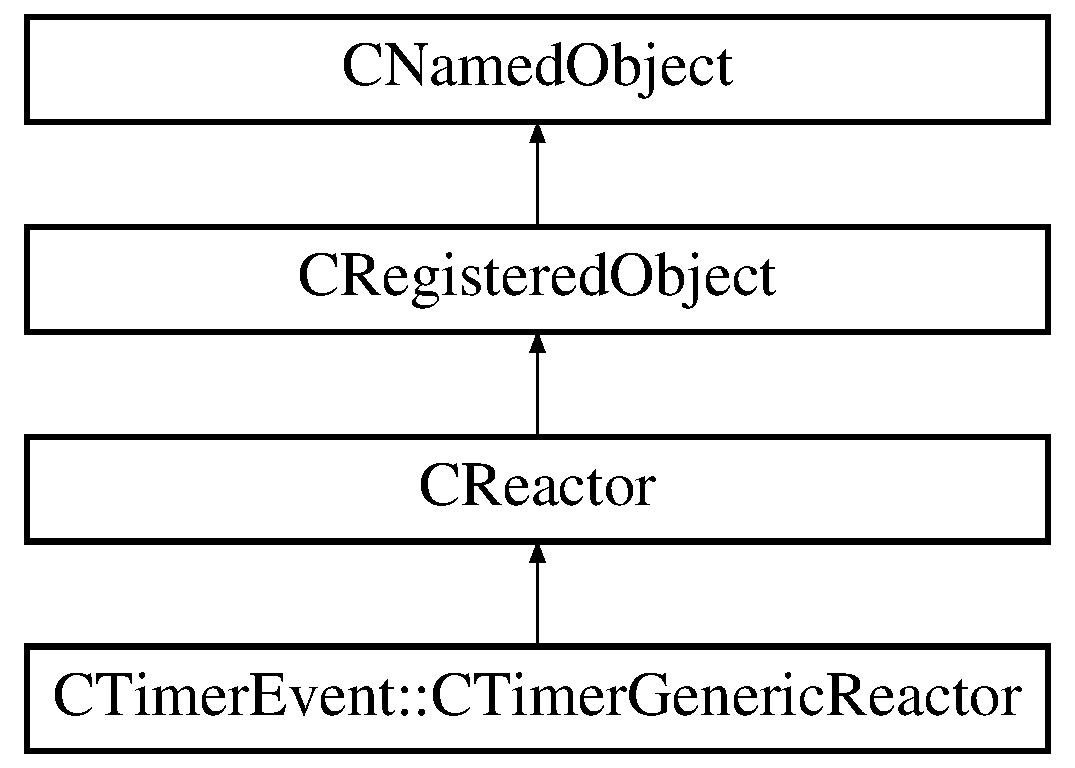
\includegraphics[height=4cm]{classCTimerEvent_1_1CTimerGenericReactor}
\end{center}
\end{figure}
\subsection*{Public Methods}
\begin{CompactItemize}
\item 
{\bf CTimer\-Generic\-Reactor} ({\bf CTimer\-Event} \&r\-Owner)
\item 
{\bf CTimer\-Generic\-Reactor} (const char $\ast$p\-Name, {\bf CTimer\-Event} \&r\-Owner)
\item 
virtual void {\bf On\-Event} ({\bf CEvent\-Monitor} \&r\-Monitor)
\end{CompactItemize}
\subsection*{Private Attributes}
\begin{CompactItemize}
\item 
{\bf CTimer\-Event} \& {\bf m\_\-r\-Owner}
\begin{CompactList}\small\item\em My Owner.\item\end{CompactList}\end{CompactItemize}


\subsection{Detailed Description}
{\bf CTimer\-Generic\-Reactor} {\rm (p.\,\pageref{classCTimerEvent_1_1CTimerGenericReactor})} - is a timer reactor which allows the timer event to look to the programmer like a monolithic entitiy. It calls the {\bf CTimer\-Event} {\rm (p.\,\pageref{classCTimerEvent})} classe's On\-Event when the timer fires. 



Definition at line 324 of file CTimer\-Event.h.

\subsection{Constructor \& Destructor Documentation}
\index{CTimerEvent::CTimerGenericReactor@{CTimer\-Event::CTimer\-Generic\-Reactor}!CTimerGenericReactor@{CTimerGenericReactor}}
\index{CTimerGenericReactor@{CTimerGenericReactor}!CTimerEvent::CTimerGenericReactor@{CTimer\-Event::CTimer\-Generic\-Reactor}}
\subsubsection{\setlength{\rightskip}{0pt plus 5cm}CTimer\-Event::CTimer\-Generic\-Reactor::CTimer\-Generic\-Reactor ({\bf CTimer\-Event} \& {\em r\-Owner})}\label{classCTimerEvent_1_1CTimerGenericReactor_a0}


Construct a generic reactor for the {\bf CTimer\-Event} {\rm (p.\,\pageref{classCTimerEvent})} class. The reactor is a callback reactor which acts to make the event class appear monolithic to anyone who users it.\begin{Desc}
\item[Parameters: ]\par
\begin{description}
\item[{\em 
const}]char$\ast$ p\-Name - Name of the reactor. \item[{\em 
{\bf CTimer\-Event} {\rm (p.\,\pageref{classCTimerEvent})}\&}]r\-Owner - The event to which I\char`\"{}ve been attached. \end{description}
\end{Desc}


Definition at line 299 of file CTimer\-Event.cpp.\index{CTimerEvent::CTimerGenericReactor@{CTimer\-Event::CTimer\-Generic\-Reactor}!CTimerGenericReactor@{CTimerGenericReactor}}
\index{CTimerGenericReactor@{CTimerGenericReactor}!CTimerEvent::CTimerGenericReactor@{CTimer\-Event::CTimer\-Generic\-Reactor}}
\subsubsection{\setlength{\rightskip}{0pt plus 5cm}CTimer\-Event::CTimer\-Generic\-Reactor::CTimer\-Generic\-Reactor (const char $\ast$ {\em p\-Name}, {\bf CTimer\-Event} \& {\em r\-Owner})}\label{classCTimerEvent_1_1CTimerGenericReactor_a1}




Definition at line 303 of file CTimer\-Event.cpp.

\subsection{Member Function Documentation}
\index{CTimerEvent::CTimerGenericReactor@{CTimer\-Event::CTimer\-Generic\-Reactor}!OnEvent@{OnEvent}}
\index{OnEvent@{OnEvent}!CTimerEvent::CTimerGenericReactor@{CTimer\-Event::CTimer\-Generic\-Reactor}}
\subsubsection{\setlength{\rightskip}{0pt plus 5cm}void CTimer\-Event::CTimer\-Generic\-Reactor::On\-Event ({\bf CEvent\-Monitor} \& {\em r\-Monitor})\hspace{0.3cm}{\tt  [virtual]}}\label{classCTimerEvent_1_1CTimerGenericReactor_a2}


This is the actual callback relay. When called, this  member function just calls m\_\-r\-Monitor's On\-Timer. On\-Timer is called because oneshot timers must be treated specailly to ensure that the thread exits. 

Reimplemented from {\bf CReactor} {\rm (p.\,\pageref{classCReactor_a6})}.

Definition at line 315 of file CTimer\-Event.cpp.

References CTimer\-Event::Internal\-On\-Timer(), and m\_\-r\-Owner.

\subsection{Member Data Documentation}
\index{CTimerEvent::CTimerGenericReactor@{CTimer\-Event::CTimer\-Generic\-Reactor}!m_rOwner@{m\_\-rOwner}}
\index{m_rOwner@{m\_\-rOwner}!CTimerEvent::CTimerGenericReactor@{CTimer\-Event::CTimer\-Generic\-Reactor}}
\subsubsection{\setlength{\rightskip}{0pt plus 5cm}{\bf CTimer\-Event}\& CTimer\-Event::CTimer\-Generic\-Reactor::m\_\-r\-Owner\hspace{0.3cm}{\tt  [private]}}\label{classCTimerEvent_1_1CTimerGenericReactor_o0}


My Owner.



Definition at line 326 of file CTimer\-Event.h.

Referenced by On\-Event().

The documentation for this class was generated from the following files:\begin{CompactItemize}
\item 
{\bf CTimer\-Event.h}\item 
{\bf CTimer\-Event.cpp}\end{CompactItemize}
